% !TEX encoding = UTF-8 Unicode
%\documentclass[a4paper,12pt,report]{jsbook}
\documentclass[a4paper,twocolumn,report,10.5pt]{jsbook}


%% いろいろパッケヌゞ %%
\usepackage{ascmac}
\usepackage{url}
\usepackage[dvipdfmx]{graphicx}
\usepackage{pifont}
\usepackage{here}   % 指定力の匷い堎所指定
\usepackage{otf}    % UTF文字指定

%% 画像蚭定 %%

% 画像グラフのディレクトリを指定
\graphicspath{{./image/}{./graph/}}

%% 数匏蚭定 %%

% 数匏数匏甚フォント
\usepackage{amsmath,amssymb,bm}	
\newcommand{\argmax}{\mathop{\rm arg~max}\limits}
\newcommand{\argmin}{\mathop{\rm arg~min}\limits}

% 定矩
\def\vector#1{\mbox{\boldmath $#1$}}

%%%% ペヌゞ蚭定 %%%%%%%%%%%%%%%%%%%%%%%%%%%%%%%%%%

%% ヘッダ・フッタの蚭定 %%

% ヘッダフッタなどに特殊なスタむルを導入するパッケヌゞ
\usepackage{fancyhdr}

% ヘッダに䞋線を入れる
\pagestyle{fancyplain}
% ヘッダの巊に節の芋出しを衚瀺
\lhead{\leftmark}
% ヘッダの右にペヌゞ番号を衚瀺
\rhead{\thepage}
% ヘッダの䞭倮
\chead{}

% フッタの巊
\lfoot{}
% フッタの右
\rfoot{}
% フッタの䞭倮
\cfoot{}

%図ず本文の䜙癜よく分からんけど空きすぎおお䞍恰奜だったので远加
\setlength\intextsep{2zw}	% 途䞭に出力される図ず本文の䜙癜
\setlength\textfloatsep{2zw}	% 図ず本文の䜙癜
\setlength\abovecaptionskip{0pt} %図ずキャプションの䜙癜
\setlength{\itemsep}{0cm}	%箇条曞きの項目間 



%% 本文の幅の蚭定 %%
%\setlength{\textwidth}{42zh}
\setlength{\textwidth}{54zh}

% 段末の行飛びを無くす
\setlength{\parskip}{0pt}
\setlength{\topskip}{\Cht}

% 章番号
\renewcommand{\chaptermark}[1]{\markboth{第\ \thechapter\ 章~#1}{}}

% subsectionも目次に衚瀺
\setcounter{tocdepth}{2}


%%%% ここから文曞の内郚 %%%%%%%%%%%%%%%%%%%%%%%%%%%%%%%%%%
\begin{document}

%%%%%%%%%%%%%%%%%%%%
%%  衚玙

\begin{titlepage}
\begin{center}

{
\fontsize{28pt}{28pt}\selectfont % フォントサむズ28pt行送り20pt




% % タむトルゎシック䜓
% {\gt
%  \vspace*{2.5zh}
%  文曞怜玢における粟床向䞊の芁因の分析ずその圱響評䟡\\ %タむトル1行目
%  \vspace{1zh}
%  % プレむリストの自動生成\\ %タむトル2行目

% \vspace{5zh}


% \fontsize{22pt}{22pt}\selectfont % フォントサむズ2pt行送り20pt
% %幎月
% 2015幎\hspace{0.5zh}2月\\% 幎月
% %所属
% \vspace{0.5zh}
% 岐阜倧孊倧孊院\hspace{1zh}工孊研究科\hspace{1zh}\\%
% \vspace{0.5zh}
% 応甚情報孊専攻\hspace{1zh}速氎・田村研究宀\\

% %名前
% \vspace{2zh}
% 原\hspace{1zh}謙介\\

% %指導教員
% \vspace{3zh}
% 指導教員\hspace{1zh}速氎\hspace{1zh}悟 \\
% \vspace{0.5zh}
%     \hspace{1zh}田村\hspace{1zh}哲嗣
% } % \gtここたで
% }

% タイトル(ゴシック体)
{\gt
\vspace*{2.5zh}
音声ドキュメント検索手法の分析と精度改善\\ %タイトル1行目

\vspace{5zh}


\fontsize{22pt}{22pt}\selectfont % フォントサイズ2pt,行送り20pt

%年月
2018年\hspace{0.5zh}3月\\% 年月
%所属
\vspace{0.5zh}
岐阜大学大学院\hspace{1zh}工学研究科\hspace{1zh}\\%
\vspace{0.5zh}
応用情報学専攻\hspace{1zh}速水・田村研究室\\

%名前
\vspace{2zh}
田口\hspace{1zh}拓明\\

\vspace{3zh}
指導教員\hspace{1zh}速水\hspace{1zh}悟 \\
\vspace{0.5zh}
    \hspace{1zh}田村\hspace{1zh}哲嗣\\
} % \gtここまで
}





\end{center}
\end{titlepage}

%%%%%%%%%%%%%%%%%%%%%%%%%%%%%%%%%%%%%%%%%%
%%  目次

\pagenumbering{roman}
\tableofcontents
\newpage
\pagenumbering{arabic}

%%%%%%%%%%%%%%%%%%%%%%%%%%%%%%%%%%%%%%%%%%
%%  本文


%  音声ドキュメント
%%%%%%%%%%%%%%%%%%%%%%%%%%%%%%%%%%%%%%%%%%%%%
% 第1章分割

\chapter{序論} % 章の見出し
\section{背景}
近年,講演の録音やニュース番組,動画などの音声情報を含むコンテンツが増加してきている.
このようなコンテンツを検索する際には通常,予め人手でタイトルや概要などのメタ情報を付与しておき,そのメタ情報を基にしてユーザの求める情報かどうかを判定し,検索結果を出力する.
一方でそのような検索手法は,人手でメタ情報を付与する必要があり,人的コストがかかるため,音声を音声認識によってテキストの形に起こし,テキスト検索技術を用いて検索する手法が提案されている.

このテキスト検索技術には,音声認識結果を利用するため,一般のテキスト検索手法とは異なる方法を用いる.例えば,音声認識結果には音声認識誤りが存在し,これらの認識誤りはその後の特徴量計算の段階で悪影響を及ぼし,音声は基本的に話し言葉で録音されるため,冗長な話し言葉の中から複数のキーワードを認識し抽出しなければならないため,それらを考慮したテキスト検索手法が必要とされる.そのため,音声認識結果を利用したテキスト検索技術に対し,多くの研究が行なわれている. 

\subsection{NTCIR}
% TODO: 参考文献
NTCIR(NII Test Collection for Information Retrieval)\cite{NTCIR}とは,膨大な情報の中から所望の情報にアクセスする技術の発展を図るプロジェクトである.
NTCIRでは研究分野に応じて情報検索,質問応答,要約,テキストマイニング,機械翻訳など,様々なタスクが用意される.
各タスクでは,評価の為のテストコレクションと,その実験結果を評価するためのツールが用意される.
タスクの参加者は,共通のテストコレクションの上で研究し,精度を競い合う.
NTCIRの目的には,次の3つが挙げられる.
\begin{enumerate}
    \item 大規模かつ再利用可能なテストコレクションの構築
    \item 多数の研究者が研究成果を提供し,相互に学び合うフォーラムの形成
    \item 情報アクセス技術と,その評価手法,評価指標に関する研究の推進
\end{enumerate}

\subsection{SpokenQuery\&Doc}
SpokenQuery\&Docでは,大量に存在する音声データからユーザに有用性のあるデータを検索する事を目的とする.本タスクでは,2種類のサブタスクから音声ドキュメントの検索を目指す.STD(Spoken Term Detection)サブタスクでは単語クエリが与えられ,大量に存在する音声ドキュメントの中から単語クエリが発話されている文書の部位を検索し,検索精度と検索にかかった時間で評価する.一方SDR(Spoken Document Retrieval)サブタスクでは質問文形式の質問クエリが与えられ,検索対象の音声ドキュメントから質問クエリの内容に該当する文書(講演単位:Lecture Retrieval)又は文書中の部位(部位単位:Passage Retrieval)を検索する.我々はSpokenDoc SDR Passage Retrievalに参加しており,本論文における音声ドキュメント検索問題とは当タスクの問題を指すこととする.

\section{研究目的}
前節で解説したSpokenDocタスクのように,音声認識結果と質問クエリが存在する場合,質問クエリを文書として見ることで,音声認識結果テキストとの類似度を検索に用いる手法が考えられる.

この検索方法において,まず音声認識精度を改善し,認識誤りが減少すれば,テキスト検索手法の精度を改善できると考えられる.そのため,本研究では精度の高い音声認識エンジンを利用し,検索精度を向上させる.

また,類似度計算の特徴量としては一般的にTF-IDF法が用いられるが,今回のSDRタスクのように質問クエリのテキストの長さが不十分な場合,TF-IDF法ではうまく推定を行う事ができない.またTF-IDF法は音声認識誤りや言い換え問題に対しても弱いため,そのまま文書検索に用いるには疑問が残る.
本研究はこれらの問題の解決を試みることで,音声ドキュメントの検索の精度向上を図る.まずTF-IDF法による文書間の類似度を用いない手法,すなわち確率的言語モデルを用いた音声ドキュメントの検索について述べる.また,確率的言語モデルとして一般的であるクエリ尤度モデル \cite{query_likelihood}について関連文書を用いた拡張を行い,その有用性について検討する.

SDRタスクにおいて,検索対象となる文書のテキストの長さが短い場合が存在し,この時テキストの情報が少ないため,テキスト検索精度が低いことがある.そのため,本研究では検索対象となる文書の周囲のテキストを利用し,検索精度の向上を図る.
周囲のテキストを利用する具体的な方法としては,キャッシュモデル・N-gram言語モデル・リカレントニューラルネットワーク言語モデルなどの,単語が出現する順序に着目した言語的特徴量を利用したり,検索対象となる文書の周囲の文書と質問クエリとの類似度スコアを統合したりする.これらの手法による音声ドキュメントの検索について考察を行う.

\section{論文構成}
\noindent
本論文の構成を以下に示す.

第2章では,音声ドキュメントの検索の基礎技術として,TF-IDF法をはじめとした自然言語処理技術について述べる.

第3章では,音声認識精度と検索精度について述べる.音声認識精度の高い認識エンジンが生成した音声ドキュメントが検索精度にどのように影響するのかを分析する.

第4章では,クエリの関連文書を用いたクエリ尤度モデルの拡張について説明する.Web文書と論文を用いて,クエリ尤度モデルを拡張する.

第5章では,文脈を考慮した言語特徴量の検討について説明する.言語特徴量として近年よく利用されるキャッシュモデル・N-gram言語モデル・リカレントニューラルネットワーク言語モデルについて,それぞれ評価し,影響を分析する.

第6章では,前後の部分文書の情報を加味した時の検索精度の改善について述べる. 

そして,第7章では提案した手法において,有効な方法を統合し,更なる検索精度の改善を目指す. 

最後に,第8章でまとめと今後の課題を述べる.

% TODO: 
% 章が確定してないため,確定次第書きます.流れとしては
% ▶︎クエリ尤度に対して,Web文書と論文文書の統合
% ▶︎クエリ尤度,クエリ尤度 + キャッシュ, クエリ尤度 + RNN のMAP値比較
% ▶︎それらの手法 + スライド統合でのMAP値
% 論文構成を以下に示す.
 % 第1ç« (chapter1.texに蚘述)

\chapter{文書検索のための自然言語処理}
本章では文書から特徴量を計算し,文書検索に応用する方法について述べる.
最初に,文章を単語列にする形態素解析について説明する.また,音声から文書を生成する音声認識について解説する.
次に,テキストマイニングの分野で広く用いられている発見的手法のTF-IDFによる文書検索手法について説明する.
そして,確率的言語モデルであるクエリ尤度モデルを用いた文書検索手法について述べる.
さらに,他の技術を用いた文書検索手法を提案する.
最後に,文書検索の評価尺度の1つであるMAP(Mean Average Precision)について説明する.

\section{形態素解析}
前処理として形態素解析を行う.
形態素とは,「ある言語において,それ以上分解すると意味をなさなくなるところまで分解して抽出された,音素のまとまりの一つ一つ」である.
日本語においては,形態素は単語と同じ意味を持つ.
形態素解析とは,与えられた文字列を形態素の列に分割し,品詞を解析する作業である.
本研究における形態素解析の目的は,単語の出現回数のカウントを可能にし,単語が名詞であるかどうかを判定することにある.
本研究では,形態素解析にMeCab\cite{MeCab}を用いた.

\subsection{MeCab}
MeCabとは, 京都大学情報学研究科-日本電信電話株式会社コミュニケーション科学基礎研究所 共同研究ユニットプロジェクトを通じて開発された
オープンソース 形態素解析エンジンである.
% 言語,辞書,コーパスに依存しない汎用的な設計を基本方針としている.
パラメータの推定にCRF(Conditional Random Fields)を用いており,隠れマルコフモデルを採用している形態素解析器のChaSen\cite{ChaSen}より
精度が向上している.
また,外部から容易に利用できるようなインターフェースを備えているため,他のシステムに組み込みやすいという特徴を持つ.

% 
% 田口追加
%

\section{音声認識}
現在の音声認識は,多くの場合確率モデルを用いた統計的手法に基づいている.従ってどのような統計的データを持つモデルを構築するかによって,音声認識結果は大きく変わることになる.音声$X$に対して,任意の単語列 $d$の中から最も適合する単語列 $d'$ を求める処理は,式(\ref{onsei_ninsiki1})として定式化される.\\

\begin{equation}
    d' = \argmax_{d} P(d|X) 
    \label{onsei_ninsiki1}
\end{equation}

% TODO: 式
ここでベイズの定理を適応すると,式(\ref{onsei_ninsiki1})は式(\ref{onsei_ninsiki2})へと変形することができる.

\begin{equation}
    d' = \argmax_{d}  \frac{P(X|d)P(d)}{P(X)} 
    \label{onsei_ninsiki2}
\end{equation}

% TODO: 式
また,$d$の最大値は分母の値に関わらないため,最終的に式(\ref{onsei_ninsiki3})のように変形される.

\begin{equation}
    d' = \argmax_{d}  P(X|d)P(d) 
    \label{onsei_ninsiki3}
\end{equation}

結果,音声認識は $P(X|d)$と$P(d)$によってモデル化されると考えることができる.$P(X|d)$は,単語列 $P(d)$に対して特徴ベクトル $X$ が観測される確率である.また,$P(d)$ は単語列$d$の言語的な生起確率である.

\subsection{音響モデル}
音響モデルとは,音素や音節の周波数パターンを用いて入力音声のマッチングを行うための確率的モデルである.式(\ref{onsei_ninsiki3})の $P(X|d)$ は単語列 $d = (w_1, w_2, ..., w_{|d|})$ に対する音響パターンが $X$ である確率を表し,音響モデルと照合することによって計算される.音響モデルはあらゆる文や単語パターンの音響確率を計算できるように音素に代表される音韻単位で用意される.すなわち単語列は音素列 $m_1, m_2, ... , m_I $ に展開され,式(\ref{onkyo_model1})で計算される.

\begin{equation}
    P(X|d) = \prod_{I}  P(X|m_i) 
    \label{onkyo_model1}
\end{equation}

ここで $P(X|m_i)$ とは音素単位の音響的特徴量を表現したモデルである.また,$x$ は入力音声の一部 $x \in X$ である.
現在広く用いられているモデルは隠れマルコフモデル(HMM: Hidden Markov Model)である.HMMは定常な信号源を確率的に切り替えていくことで,時々刻々と変化する非定常信号を表現する.

\subsection{統計的言語モデル}

言語モデルとは,式(\ref{onsei_ninsiki3})の $P(d)$ にあたる,単語の生起確率を与えるモデルである.統計的なモデルに基づく言語モデルの場合,推定対象となる単語を前にある単語との接続情報から推定する.このとき文の先頭からの全ての単語の接続情報を考慮するのが理想であるが,現在では単語の直前 $N-1$ 単語の接続情報で近似する手法が一般的であり,この手法はN-gramと呼ばれる.以下にN-gramの説明を示す. 
 $N$ 個の単語の接続を確率として表すと,式(\ref{onkyo_model2})のように示される.

\begin{equation}
    P(w_i|w_{i-N+1}, ..., w_{i-1})) = \frac{ c(w_{i-N+1}, ..., w_{i-1}) }{ c(w_{i-N+1}, ..., w_{i-1}, w_i) }  
    \label{onkyo_model2}
\end{equation}

ここで $c(w_{i-N+1}, ..., w_{i-1})$ は単語列 $w_{i-N+1}, ..., w_{i-1}$ が同時生起する頻度である.日本語の文章は単語の定義が明確でないため,予め形態素解析を行いひとつの単語を単位としてN-gramを構成することが一般的である. 
N-gramを構成する際の問題点として,「文法的には正しいが,偶然にもテキスト内に1回も出現しない」単語が出現した場合,N-gramが存在しないため確率を推定することができない.また,「大量に存在するテキスト内に,1回しか出現しない」単語のN-gramがほぼ0となり,そのような単語は大量に存在するので,計算コストが必要以上に増加してしまう.これらの問題の解決法として,頻出単語以外の単語を未知語として処理する,スムージングが挙げられる.スムージングを行うことにより,計算時間を減らしつつN-gram構築時に一度も出現しなかった単語の組み合わせの生起確率を推定することができる.


%
% 田口 END
%

% TODO: TFの説明とか追加しても良い

\section{TF-IDFを用いた文書検索} \label{sec_tfidf}
本節では,クエリのTF-IDFベクトルと文書のTF-IDFベクトルを比較する手法について述べる.
\subsection{ユークリッド距離}
% TODO:ユークリッド距離の図,欠点が分かるように
ユークリッド距離は,ベクトル空間上の2ベクトルの距離である.
ベクトル空間上の2ベクトル$X = {x_1, x_2, ..., x_d}, Y = {y_1, y_2, ..., y_d}$が存在したとき,
ユークリッド距離$Euc(X, Y)$は式(\ref{eq_euc})で計算される.
\begin{equation}
    Euc(X, Y) = \sqrt{\sum^{d}_{i=1}{x_i^2 - y_i^2}}    \label{eq_euc}
\end{equation}
ユークリッド距離は,ベクトルの角度だけでなく,ベクトルの大きさによっても変わる.
すなわちTF-IDFのような文書ベクトルを比較する際には,文書長によっても類似度が変化する.
そのため文書検索においては,1クエリに対して長さが異なる2つ以上の文書を比較すると,正しく類似度を計算することができない問題がある.

\subsection{コサイン類似度} \label{sec_cosine}
% TODO:コサイン類似度の図
コサイン類似度は,ユークリッド距離と同じく,2つのベクトルの類似度を計る手法の一つである.
コサイン類似度は,2つのベクトル$X = {x_1, x_2, ..., x_d}, Y = {y_1, y_2, ..., y_d}$が存在したとき,
$X, Y$の成す角度$\theta$が小さいほど類似度$cos(\theta)$が高いとする手法であり,式(\ref{eq_cos})で計算される.
\begin{equation}
    cos(\theta) = \frac{X \cdot Y}{|X||Y|}  \label{eq_cos}
\end{equation}
コサイン類似度はベクトルの長さに依存せず,角度のみで類似度を計算する.
そのため,TF-IDFのような文書ベクトルの比較の際に,それぞれのベクトルの大きさ,すなわち文書長に依存しないため,
ユークリッド距離よりも類似度比較に優れているとされる.

\subsection{クエリ尤度モデル}
情報検索は,クエリと検索対象の文書群が与えられた時に,クエリに適合する度合いにしたがって文書をランキングする問題と言い換えることができる.
すなわち,文書$D$がクエリ$Q$に適合する確率$P(D|Q)$を最大にする$D$を求める問題である.
これをベイズの定理を用いて変形すると,式(\ref{eq_query_likelihood1})となる.
\begin{equation}
    \argmax_{D} P(D|Q) = \argmax_{D} \frac{P(Q|D)P(D)}{P(Q)}    \label{eq_query_likelihood1}
\end{equation}
式(\ref{eq_query_likelihood1})において,$P(Q)$はクエリの生成確率分布であるが,文書$D$に依存しないため定数とみなすことができる.
また,$P(D)$は文書の生成確率分布であるが,どのような文書が与えられるかという事前知識が無い限り,一様であるとみなさざるを得ない.
よって式(\ref{eq_query_likelihood1})は式(\ref{eq_query_likelihood2})となる.
\begin{equation}
    \argmax_{D} P(D|Q) = \argmax_{D} P(Q|D) \label{eq_query_likelihood2}
\end{equation}
式(\ref{eq_query_likelihood2})の右辺は,文書に関する言語モデルがクエリを生成する確率$P(Q|D)$を表している.
これに基づく文書検索手法を,クエリ尤度モデルと呼ぶ.

クエリ尤度モデルにおいて文書を言語モデル化する際,ユニグラム言語モデルが頻繁に用いられる.
ユニグラム言語モデルは,語が周辺の語に依らず独立に生起するという仮定に基づいている.
ユニグラム言語モデルを$|\theta_D|$から$|Q|$個の語から成るクエリ$Q = \{q_1, q_2, ..., q_|Q|\}$が生成される尤度$P(Q|D)$は,式(\ref{eq_unigram})で計算される.
\begin{equation}
    P(Q|D) = \prod^{Q}_{l=1}P(q_l|\theta_d) \label{eq_unigram}
\end{equation}
ここで,クエリ$Q$中において,の語彙$V = \{w_1, w_2, ..., w_|V|\}$が複数回出現する可能性を考慮すると,式(\ref{eq_unigram})は式(\ref{eq_unigram2})と変形できる.
\begin{equation}
    P(Q|D) = \prod^{Q}_{w_i \in V}P(w_i|\theta_d)^{c(w_i, Q)} \label{eq_unigram2}
\end{equation}
ここで$c(w_i, Q)$はクエリ$Q$において語$w_i$が出現した回数である.
このように,クエリ尤度モデルによる文書検索問題は,$P(w_i|\theta_d)$の推定問題に帰着する.

本研究では,文書モデル$\theta_d$の推定方法に,文書中の語の相対頻度を用いた.
$P(w_i|\theta_d)$は式(\ref{eq_wordprob})で計算される.
\begin{equation}
    P(w_i|\theta_d) = \frac{c(w_i,D)}{|D|}    \label{eq_wordprob}
\end{equation}
ここで$c(w_i,D)$は文書$D$中の単語の出現回数を表し,$|D|$は文書$D$の単語数を表す.
これは文書における単語が観測された状況における,多項分布のパラメータの最尤推定に他ならない.

\subsection{ディリクレスムージング}  \label{sec_dirichlet}
式(\ref{eq_unigram})において,文書中に出現しない語,すなわち出現確率が0の語が1つでもクエリ中に存在すると,尤度が0となってしまう.
その場合,クエリ語が1つも存在しない文書と,クエリ語を一部含む文書との比較ができなくなる.これを零確率問題と呼ぶ.
また,文書長が短い場合には,式(\ref{eq_wordprob})では正しくモデルを推定することが出来ない.
これらの問題に対処するために,文書モデルのスムージングが行われる.
スムージングとは,何らかの方法で文書に含まれない語に微小の確率を割り振ることである.
これにより質問クエリに存在しない語を含む文書に対しては式(\ref{eq_unigram})に従ってそれらの微小な確率値が掛け合わされ,
結果としてクエリ尤度の値が小さくなり,前述の零確率問題に対処することができる.

本研究ではスムージングに,ディリクレスムージングを用いた.
ディリクレスムージングは,ディリクレ分布を文書多項分布の事前知識として導入するものであり,式(\ref{eq_dirichlet})によって計算される.
\begin{equation}
    P(w_i|\theta_d;\mu) = \frac{ c(w_i, D) + \mu P(w_i|\theta_C) }{ |D| + \mu } \label{eq_dirichlet}
\end{equation}
ここで,$\mu$はディリクレ事前分布のパラメータであり,正の値を持つ.また,$\theta_C$はディリクレスムージングのための文書コレクションから
推定された文書モデルである.
式(\ref{eq_dirichlet})を式(\ref{eq_wordprob})の拡張になるように変形すると,式(\ref{eq_dirichlet2})となる.
\begin{equation}
    P(w_i|\theta_d;\mu) = \frac{|D|}{|D|+\mu} \frac{c(w_i, D)}{|D|} + \frac{\mu}{|D|+\mu}P(w_i|\theta_C)  \label{eq_dirichlet2}
\end{equation}
式(\ref{eq_dirichlet2})によれば,補完の度合い$\frac{\mu}{|D|+\mu}$が文書長$|D|$によって補完の度合いが変化する.
これは長い文書ほど文書中の単語の観測サンプル数が大きくなるためにスムージングの必要性が低くなり,
逆に短い文書ほど必要性が高くなることを反映しており,前述の短い文書においてクエリ語が存在しない問題を解決している.

\section{MAP} \label{sec_map}
SpokenQuery\&Docの評価尺度にはMAP(Mean Average Precision)が用いられている.
これはクエリ毎の平均適合率AP値の平均である.
クエリ$q$に対するAP値$AP(q)$は式(\ref{eq_ap})で計算される.
\begin{equation}
    AP(q) = \frac{1}{|N|} \sum^N_{i=1} \frac{i}{rank(i)}    \label{eq_ap}
\end{equation}
ここで$N$はクエリ$q$に対する正解文書の数,$rank(i)$はクエリ$q$の$i$番目の正解文書が,文書検索によって付けられた順位である.
AP値,MAPは共に[0, 1]の値をとる.


\chapter{単語のベクトル表現}
本章では単語をベクトルで表現する技術について解説する.
まず最も簡単な1-of-K表現について述べ,次に2単語のベクトル間距離が近いほど,意味も近いとする,単語の分散表現について述べる.
その後,単語の分散表現を学習するために用いるニューラルネットワークについて説明し,
実際に単語の分散表現を学習するツールであるword2vecのアルゴリズムについて解説する.

\section{1-of-K表現}
1-of-K表現とは,語彙が$K$単語存在するとき,単語をK次元かつ長さが1である,2値ベクトルで表現したものである.
このベクトル表現では,異なる任意の2単語のユークリッド距離が全て等しいという特徴を持つ.
単語間の距離を意味の近さと捉えたとき,この表現方法は現実的ではないという問題がある.
\section{単語の分散表現}
単語の分散表現とは,1-of-Kベクトルの情報を,もっと低い次元の実数ベクトルで表現したものである.
単語の分散表現を作る方法はいくつか存在するが,
後述するword2vecでは,ニューラルネットワークを用いて1-of-K表現から単語の分散表現を学習する.
1-of-K表現では単語が全て等距離であったが,単語の分散表現では単語間の距離が単語の意味的な距離になることが期待できる.

\section{ニューラルネットワーク}
% 中間層,出力層
本節ではword2vecで用いられるニューラルネットワークの基礎について説明する.
ニューラルネットワークは生物の神経細胞(ニューロン)を参考に作られたモデルであり,
$N$入力$M$出力(ただし,$N, M$は自然数)のベクトル写像である.
ニューラルネットワークは複数の形式ニューロンによって構成され,形式ニューロンの出力が別の形式ニューロンの入力になるように構成されている.
\subsection{形式ニューロン}
形式ニューロンは,$N$入力1出力のベクトル写像である.
形式ニューロンは$N$個の入力から1つの数値$y^{IN}$を計算し,それを形式ニューロンの持つ活性化関数$f$への入力とする.
形式ニューロンの出力$y^{OUT}$は,$y^{IN}$に活性化関数$f$へ適用したものとなる.
\begin{equation}
    y^{OUT} = f(y^{IN}) \label{eq_neuron}
\end{equation}
形式ニューロンには,$N$個の入力毎に決められた重み$w=(w_1, w_2, ..., w_N)$が与えられている.
形式ニューロンへの入力$x$が$x=(x_1, x_2, ..., x_N)$のとき,活性化関数への入力$y^{IN}$は式(\ref{eq_yin})で計算される.
\begin{equation}
    y^{IN} = wx^T = \sum^N_{i=1}w_ix_i \label{eq_yin} 
\end{equation}

% 活性化関数
出力層の活性化関数にはソフトマックス関数が一般的に用いられおり,word2vecにおいてもソフトマックスを簡易化したものが用いられている.
ソフトマックス関数は式(\ref{eq_softmax})で計算される.
\begin{equation}
    y_i^{OUT} = \frac{exp(y_i^{IN})}{\sum_k exp(y_k^{IN})}  \label{eq_softmax}
\end{equation}

\section{word2vec}
word2vec\cite{word2vec}とは,形態素に分かち書きされた文章から,ニューラルネットワークを用いて単語の分散表現を学習する手法およびツールである.
word2vecでは,文章中のある注目単語の前後$n$単語に出現する語は互いに関係があるという仮定に基づいて,単語の分散表現を学習する.
word2vecで単語の分散表現を学習する際には,CBOW(Continuous Bag-of-Words)とSkip-gramの,どちらかのニューラルネットワークを用いて学習する.
また本研究ではword2vecのモデルに,CSJ(Corpus of spontaneous Japanese, 日本語話し言葉コーパス)を用いて学習したモデルと,
NTCIR11 SpokenQuery\&Docの検索対象文書から,\ref{sec_webquery}に倣って取得したWeb文書から学習したモデルの2つを用いている.
\subsection{CBOW}
CBOWでは,注目単語の前後$n$単語のBag-of-Wordsを入力とし,注目単語を出力するニューラルネットワークを学習する.
ここでBag-of-Wordsとは,単語の1-of-K表現を足し合わせたものを表すものとする.
CBOWでは計算の高速化のために,中間層の活性化関数には恒等写像を用いている.
また,入力層から隠れ層への入力の重み$w$が全て均一の値になっている.
\subsection{Skip-gram}
Skip-gramでは,ある注目単語1つの1-of-Kが与えられた時,その前後$n$単語のBag-of-Wordsを出力とするニューラルネットワークを学習する.


\chapter{文書の比較方法}
本章では文書から特徴量を計算し,文書検索に応用する方法について述べる.
まず初めに,テキストマイニングの分野で広く用いられている発見的手法のTF-IDFによる文書検索手法と,
TF-IDFによる文書検索手法を改良したBM25について説明する.
次に確率的言語モデルであるクエリ尤度モデルを用いた文書検索手法について述べる.
さらに,他の技術を用いた文書検索手法を提案する.
\section{TF-IDFを用いた文書検索}
本節では,クエリのTF-IDFベクトルと文書のTF-IDFベクトルを比較する手法について述べる.
\subsection{ユークリッド距離}
% TODO:ユークリッド距離の図,欠点が分かるように
ユークリッド距離は,ベクトル空間上の2ベクトルの距離である.
ベクトル空間上の2ベクトル$X = {x_1, x_2, ..., x_d}, Y = {y_1, y_2, ..., y_d}$が存在したとき,
ユークリッド距離$Euc(X, Y)$は式(\ref{eq_euc})で計算される.
\begin{equation}
    Euc(X, Y) = \sqrt{\sum^{d}_{i=1}{x_i^2 - y_i^2}}    \label{eq_euc}
\end{equation}
ユークリッド距離は,ベクトルの角度だけでなく,ベクトルの大きさによっても変わる.
すなわちTF-IDFのような文書ベクトルを比較する際には,文書長によっても類似度が変化する.
そのため文書検索においては,1クエリに対して長さが異なる2つ以上の文書を比較すると,正しく類似度を計算することができない問題がある.

\subsection{コサイン類似度} \label{sec_cosine}
% TODO:コサイン類似度の図
コサイン類似度は,ユークリッド距離と同じく,2つのベクトルの類似度を計る手法の一つである.
コサイン類似度は,2つのベクトル$X = {x_1, x_2, ..., x_d}, Y = {y_1, y_2, ..., y_d}$が存在したとき,
$X, Y$の成す角度$\theta$が小さいほど類似度$cos(\theta)$が高いとする手法であり,式(\ref{eq_cos})で計算される.
\begin{equation}
    cos(\theta) = \frac{X \cdot Y}{|X||Y|}  \label{eq_cos}
\end{equation}
コサイン類似度はベクトルの長さに依存せず,角度のみで類似度を計算する.
そのため,TF-IDFのような文書ベクトルの比較の際に,それぞれのベクトルの大きさ,すなわち文書長に依存しないため,
ユークリッド距離よりも類似度比較に優れているとされる.

\subsection{Webクエリ拡張}   \label{sec_webquery}
2文書をTF-IDFベクトルで比較する場合,文書中に存在しない語について比較できない.
また本研究で扱う文書検索の問題において,一般にクエリは短く,少語彙であることが多い.
すなわち,クエリの持つ語が少ないために,比較がうまく行えない場合がある.
また入力が音声クエリの場合,音声認識誤りによって認識が正しく行われず,本来の意図とは違う意味のクエリになる可能性がある.
これらの問題に対処するために,クエリのTF-IDFベクトルをWeb文書を用いて補完する,Webクエリ拡張を行う.

Webクエリ拡張は,クエリに関連すると考えられる文書を用いて,クエリの語彙を補完する手法である.
まず原文クエリからTF-IDFを計算し,TF-IDF上位$n$件の単語を抽出することで,原文クエリのキーワードを得る.
次にこれらの語からYahooの検索エンジンに入力するためのWeb検索クエリを生成する.
Web検索クエリは,クエリから得られた上位$n$件の単語を用いてできる,全ての3単語の組み合わせを,スペース区切りにしたものである.
すなわち,Web検索クエリは$_n C _3$組できる.
また本研究では1検索クエリあたりの取得Webページ数は100とした.
Web検索にキーワード1単語を用いず,3単語で検索するのは,Web検索で得られる文書がよりクエリと類似する文書が得られると考えられるからである.
最後に得られたWeb文書全てを,1つの巨大な文書とみなし,TF-IDFのベクトルを計算する.
最後に,原文クエリのTF-IDFと,得られたWeb文書のTF-IDFのを重み付け線型結合することにより,Webクエリ拡張されたTF-IDFベクトルを得る.
Web文書には一般的に原文クエリよりも多くの語が含まれていると考えられる.そのため,Web文書から計算されたTF-IDFを原文クエリのTF-IDFに
加味することにより,原文クエリの少語彙性を克服することができると考えられる.

\subsection{クエリ尤度モデル}
情報検索は,クエリと検索対象の文書群が与えられた時に,クエリに適合する度合いにしたがって文書をランキングする問題と言い換えることができる.
すなわち,文書$D$がクエリ$Q$に適合する確率$P(D|Q)$を最大にする$D$を求める問題である.
これをベイズの定理を用いて変形すると,式(\ref{eq_query_likelihood1})となる.
\begin{equation}
    \argmax_{D} P(D|Q) = \argmax_{D} \frac{P(Q|D)P(D)}{P(Q)}    \label{eq_query_likelihood1}
\end{equation}
式(\ref{eq_query_likelihood1})において,$P(Q)$はクエリの生成確率分布であるが,文書$D$に依存しないため定数とみなすことができる.
また,$P(D)$は文書の生成確率分布であるが,どのような文書が与えられるかという事前知識が無い限り,一様であるとみなさざるを得ない.
よって式(\ref{eq_query_likelihood1})は式(\ref{eq_query_likelihood2})となる.
\begin{equation}
    \argmax_{D} P(D|Q) = \argmax_{D} P(Q|D) \label{eq_query_likelihood2}
\end{equation}
式(\ref{eq_query_likelihood2})の右辺は,文書に関する言語モデルがクエリを生成する確率$P(Q|D)$を表している.
これに基づく文書検索手法を,クエリ尤度モデルと呼ぶ.

クエリ尤度モデルにおいて文書を言語モデル化する際,ユニグラム言語モデルが頻繁に用いられる.
ユニグラム言語モデルは,語が周辺の語に依らず独立に生起するという仮定に基づいている.
ユニグラム言語モデルを$|\theta_D|$から$|Q|$個の語から成るクエリ$Q = \{q_1, q_2, ..., q_|Q|\}$が生成される尤度$P(Q|D)$は,式(\ref{eq_unigram})で計算される.
\begin{equation}
    P(Q|D) = \prod^{Q}_{l=1}P(q_l|\theta_d) \label{eq_unigram}
\end{equation}
ここで,クエリ$Q$中において,の語彙$V = \{w_1, w_2, ..., w_|V|\}$が複数回出現する可能性を考慮すると,式(\ref{eq_unigram})は式(\ref{eq_unigram2})と変形できる.
\begin{equation}
    P(Q|D) = \prod^{Q}_{w_i \in V}P(w_i|\theta_d)^{c(w_i, Q)} \label{eq_unigram2}
\end{equation}
ここで$c(w_i, Q)$はクエリ$Q$において語$w_i$が出現した回数である.
このように,クエリ尤度モデルによる文書検索問題は,$P(w_i|\theta_d)$の推定問題に帰着する.

本研究では,文書モデル$\theta_d$の推定方法に,文書中の語の相対頻度を用いた.
$P(w_i|\theta_d)$は式(\ref{eq_wordprob})で計算される.
\begin{equation}
    P(w_i|\theta_d) = \frac{c(w_i,D)}{|D|}    \label{eq_wordprob}
\end{equation}
ここで$c(w_i,D)$は文書$D$中の単語の出現回数を表し,$|D|$は文書$D$の単語数を表す.
これは文書における単語が観測された状況における,多項分布のパラメータの最尤推定に他ならない.

\subsection{ディリクレスムージング}  \label{sec_dirichlet}
式(\ref{eq_unigram})において,文書中に出現しない語,すなわち出現確率が0の語が1つでもクエリ中に存在すると,尤度が0となってしまう.
その場合,クエリ語が1つも存在しない文書と,クエリ語を一部含む文書との比較ができなくなる.これを零確率問題と呼ぶ.
また,文書長が短い場合には,式(\ref{eq_wordprob})では正しくモデルを推定することが出来ない.
これらの問題に対処するために,文書モデルのスムージングが行われる.
スムージングとは,何らかの方法で文書に含まれない語に微小の確率を割り振ることである.
これにより質問クエリに存在しない語を含む文書に対しては式(\ref{eq_unigram})に従ってそれらの微小な確率値が掛け合わされ,
結果としてクエリ尤度の値が小さくなり,前述の零確率問題に対処することができる.

本研究ではスムージングに,ディリクレスムージングを用いた.
ディリクレスムージングは,ディリクレ分布を文書多項分布の事前知識として導入するものであり,式(\ref{eq_dirichlet})によって計算される.
\begin{equation}
    P(w_i|\theta_d;\mu) = \frac{ c(w_i, D) + \mu P(w_i|\theta_C) }{ |D| + \mu } \label{eq_dirichlet}
\end{equation}
ここで,$\mu$はディリクレ事前分布のパラメータであり,正の値を持つ.また,$\theta_C$はディリクレスムージングのための文書コレクションから
推定された文書モデルである.
式(\ref{eq_dirichlet})を式(\ref{eq_wordprob})の拡張になるように変形すると,式(\ref{eq_dirichlet2})となる.
\begin{equation}
    P(w_i|\theta_d;\mu) = \frac{|D|}{|D|+\mu} \frac{c(w_i, D)}{|D|} + \frac{\mu}{|D|+\mu}P(w_i|\theta_C)  \label{eq_dirichlet2}
\end{equation}
式(\ref{eq_dirichlet2})によれば,補完の度合い$\frac{\mu}{|D|+\mu}$が文書長$|D|$によって補完の度合いが変化する.
これは長い文書ほど文書中の単語の観測サンプル数が大きくなるためにスムージングの必要性が低くなり,
逆に短い文書ほど必要性が高くなることを反映しており,前述の短い文書においてクエリ語が存在しない問題を解決している.

\subsection{Web文書を用いたディリクレスムージングの拡張} \label{sec_expanddirichlet}
本研究ではディリクレスムージングのための文書コレクションとして,検索対象の文書群を用いる.
しかし\ref{sec_webquery}節で述べたように,クエリに関連のある文書群を検索に用いることで,
クエリに対する言語モデルの表現力が向上し,より検索精度を向上させることができることが先行研究よりわかっている.
そこで本研究ではWeb文書を用いたディリクレスムージングの拡張を行う.
本手法では固定文書コレクション$\theta_C$と動的文書コレクション$\theta_W$の2つを用意し,それぞれを用いて文書モデルを作成し,スムージングに用いる.
ここでは固定文書コレクションに検索対象の文書群を,動的文書コレクションに\ref{sec_webquery}で述べた手法で収集されたWeb文書群を用いる.
式(\ref{eq_expanddirichlet})に本手法によってスムージングが行われたクエリ尤度モデルの式を示す.
\begin{flalign}
    & P(w_i|\theta_C; \mu; \nu) = \nonumber \\ 
    & \frac{|D|}{|D|+\mu+\nu}\frac{c(w_i, D)}{|D|} + \frac{\mu}{|D|+\mu+\nu}P(w_i|\theta_C) & \nonumber \\
    & + \frac{\nu}{|D|+\mu+\nu}P(w_i|\theta_W)  \label{eq_expanddirichlet}
\end{flalign}
ここで$P(w_i|\theta_W)$はWeb文書集合$W$内での語の生起確率であり,$\nu$はディリクレスムージングのパラメータであり,正の値を取る.

\subsection{LDAを用いたWeb文書の重み付けの拡張}
\ref{sec_expanddirichlet}節で収集したWeb文書群には,重要な情報を含む文書もあれば,あまり有用な情報を持っていない文書も存在すると考えられる.
そこで,より重要な情報を持つWeb文書に対しては,スムージングの際により大きな重みを持たせることで検索精度が向上することがわかっている.
本研究では検索対象文書のトピックに近い文書ほど重要な情報を持っているとして大きな重みを持たる.
まずWeb文書と検索対象文書それぞれに対して,LDA(Latent Dirichlet Allocation)を用いてトピック混合比ベクトル
$\gamma = \{\gamma_1, \gamma_2, ..., \gamma_|Z| \}$を計算する.
ここでLDAとはトピックモデルの1つであり,文書中に$|Z|$個の潜在トピック$Z = (z_1, z_2, ..., z_|Z|)$が存在すると仮定した言語モデルである.
% 文書中の潜在トピック$Z = (z_1, z_2, ..., z_|Z|)$の生成確率$\theta = (\theta_1, \theta_2, ..., \theta_|Z|)$が

その後,Web文書$W_i \in W$と検索対象文書$D_m \in D$のトピックの類似度$\sigma(W, D_m)$を,全ての検索対象文書$D$に対してコサイン類似度を用いて計算する.
その後,類似度の平均$\sigma(W_i | D)$をそのWeb文書の重みとする.
\begin{equation}
    \sigma(W_i | D) = \frac{1}{|D|}\sum^{|D|}_{m=1}\sigma(W_i, D_m) \label{eq_webweight}
\end{equation}
最後に計算された重み$\sigma(W_i | D)$を用いて,Web文書における語$w_i$の生起確率$P(w_i|\theta_W)$を式(\ref{eq_webprob})で計算する.
\begin{equation}
    P(w_i|\theta_W) = \frac{ \sum^{|W|}{l=1}\sigma(W_l, D)c(w_i, W_l) }{ \sum^{w}_{i=1} \sum^{|W|}{l=1}\sigma(W_l, D)c(w_i, W_l)}   \label{eq_webprob}
\end{equation}
ここで$w = {w_1, w_2, ..., w_|w|}$はWeb文書集合$W$中に出現する総単語数である.

\section{単語の意味的情報を用いた文書検索手法}  \label{sec_word2vec}
% \begin{itemize}
%     \item Word2vecは単語の持つ意味をベクトル空間上に表現する.
%     \item Word2vecは「ある単語の周辺にある語はお互いに近い意味を持つ」という仮定をもとにしている.
%     \item Word2vecはContinuous bag-of-wordsまたはskip-gramにより,単語の意味を表現する.(これらの違いは何か?)
%     \item 単語の意味の足し算,引き算が可能である.(King - man + woman = queen)
%     \item 学習は,線形ロジスティック回帰で行う.(これはどういったロジックなのか?)
%     \item 学習は形態素に分かち書きされた平文テキストを入力とし,予め指定した次元数で単語をベクトル空間で表現するように行われる.
%     \item 次元数の最適値は,学習コーパスの述べ単語数に比例することが先行研究で知られている.
%     \item 本研究では,CSJ(Corpus of spontaneous Japanese, 日本語話し言葉コーパス)と,NTCIR11 SpokenQuery\&Docのコーパス中の語を
%           Web検索キーワードとして取得したWeb文書を,Word2vecの学習コーパスとして用いた.
% \end{itemize}
%
本節では単語の意味的情報を考慮して文書ベクトルを生成し,比較する手法について述べる.
本手法ではまず,文書中の語に対してTF-IDFを計算し,値が上位の単語5件を,文書のキーワードとして取り出す.
次に抽出した単語5個それぞれに対してword2vecを用いて意味的情報を考慮したベクトルを割り当てる.
その後,ベクトルを平均することにより,文書の意味的情報を考慮したベクトルを生成する.
クエリと検索対象文書に対して,文書ベクトルを計算し,\ref{sec_cosine}節で述べたコサイン類似度で比較することによって文書検索を行う.

% まず,文書中の単語全てに対してWord2vecを用いてベクトルを割り当てる.
% 次に単語の位置情報を保存するために,近辺2単語のベクトルを用いて畳み込みを行う.
% その後,畳み込みが行われたベクトル群の各次元の最大値を取り出

% 本研究では文書中の単語から文書ベクトルを計算する手法として,Convolutional way\cite{convolutionalway}を用いる.
% Convolutional wayは,何らかの方法で単語に単語ベクトルを割り当て,その単語ベクトルから文書ベクトルを生成する方法である.


% %%%%%%%%%%%
% chapter2からのコピペ
%
\chapter{音声文書中の認識誤り単語の棄却手法}

音声認識結果には音声認識誤りが含まれる.これらの認識誤りは,その後の特徴量計算の段階で悪影響を及ぼし,
最終的に文書検索精度を劣化させる原因となる.
本節では音声認識結果から,単語の文脈一貫性の観点から認識誤り単語を推定し,棄却する手法を述べる.
%
% TODO:どこかにベクトル空間モデルに基づく文書比較についての話を

% TODO:卒論からのコピーなので,一部咬み合わない,上と重複する部分がある.

\section{単語の文脈一貫性に基づく誤り単語の棄却}  \label{sec_word_rejection}
% TODO:誤り単語が周辺と脈絡なく...要出典,要図
音声認識誤り単語は一般にその周辺の単語と脈絡なく現れ,関連が弱いという特徴がある.
そこで本研究では前述のPMIを用いて,単語と文書の関連度を推定し,関連が弱い語を認識誤り単語として棄却する枠組みを提案する.
文書$d = {w_1, w_2, ..., w_i, ..., w_n}$と,$d$中の単語$w_i$の関連度を,式(\ref{eq_sumpmi})で計算される$sumPMI(w_i)$で推定する.
\begin{equation}
    sumPMI(w_i) = \sum^{n}_{j=1, j \neq i}{PMI(w_i, w_j)}   \label{eq_sumpmi}
\end{equation}
PMIは2単語間の関連の強さを表すため,$sumPMI(w_i)$は単語$w_i$と文書$d$の関連の強さを表すと考えられる.
$sumPMI$が低い語は,文書との関連が弱い語であり,認識誤り単語であることが期待できる.
本研究では,$sumPMI(w)$の値が負となる単語$w$を,認識誤り単語として除外した.



%%%%%%%%%%%%%%%%%%%%%%%%%%%%%%%%%%%%%%%%%%%%%
%第5章

\chapter{実験} % 章の見出し
本章では,以下の4点に関して実際に文書検索精度を比較することで,
どのように精度が変化するかを調査・分析する.
\begin{itemize}
    \item TF-IDFにおけるTFの正規化                
    \item 単語の意味的情報の加味                  
    \item 部分文書検索における文書全体の情報の加味
    \item 音声認識誤りの棄却                      
\end{itemize}

\section{実験条件}
\begin{table}[htbp]
    \begin{center}
        \caption{実験条件}
        \begin{tabular}{|c|c|}
            \hline
            全体文書数 & 98文書 \\ \hline
            部分文書数 & 2807文書 \\ \hline
            クエリ数 & 35個 \\ \hline
            word2vec学習コーパス & Web文書 述べ語数14億語 \\ \hline
            PMI学習コーパス & 日本語話し言葉コーパス CSJ \\ \hline
        \end{tabular}
        \label{t_condition}
    \end{center}
\end{table}
実験は,NTCIR11 SpokenQuery\&Doc Formal-run の SQSCR SGS retrieval条件で行った.
実験条件を表\ref{t_condition}に示す.
特に指定しない限り,以下の実験ではクエリ・文書共に音声を人手で書き起こした条件で行った.
評価尺度にはMAPを用いた.これはクエリ毎の平均適合率AP値の平均である.クエリ$q$に対するAP値$AP(q)$は式(\ref{eq_ap})で計算される.
\begin{equation}
    AP(q) = \frac{1}{N} \sum^N_{i=1} \frac{i}{rank(i)}    \label{eq_ap}
\end{equation}
ここで$N$はクエリ$q$に対する正解文書の数,$rank(i)$はクエリ$q$の$i$番目の正解文書が,文書検索によって付けられた順位である.
AP値,MAPは共に[0, 1]の値をとる.

\section{実験結果}
\begin{table}[htbp]
    \begin{center}
        \caption{書き起こしを用いた文書検索精度}
        \begin{tabular}{|c|l|}
            \hline
            & MAP \\ \hline
            TF-IDF & 0.1629 \\ \hline \hline
            log\_TF-IDF & 0.1630 \\ \hline
            BM25 & 0.1880 \\ \hline
            word2vec & 0.1057 \\ \hline
            global & 0.2745 \\ \hline
        \end{tabular}
        \label{t_text}
    \end{center}
\end{table}
実験結果を表\ref{t_text}に示す.なお表中のword2vecはword2vecを用いた文書検索法であり,
globalはTF-IDFによる文書検索の結果に,文書全体の情報を加味したものである.
なお,$\alpha$は0.1刻みで0.1から0.9まで変化させた.

\subsection{TF-IDFにおけるTFの正規化}
\begin{figure}
    \centering
    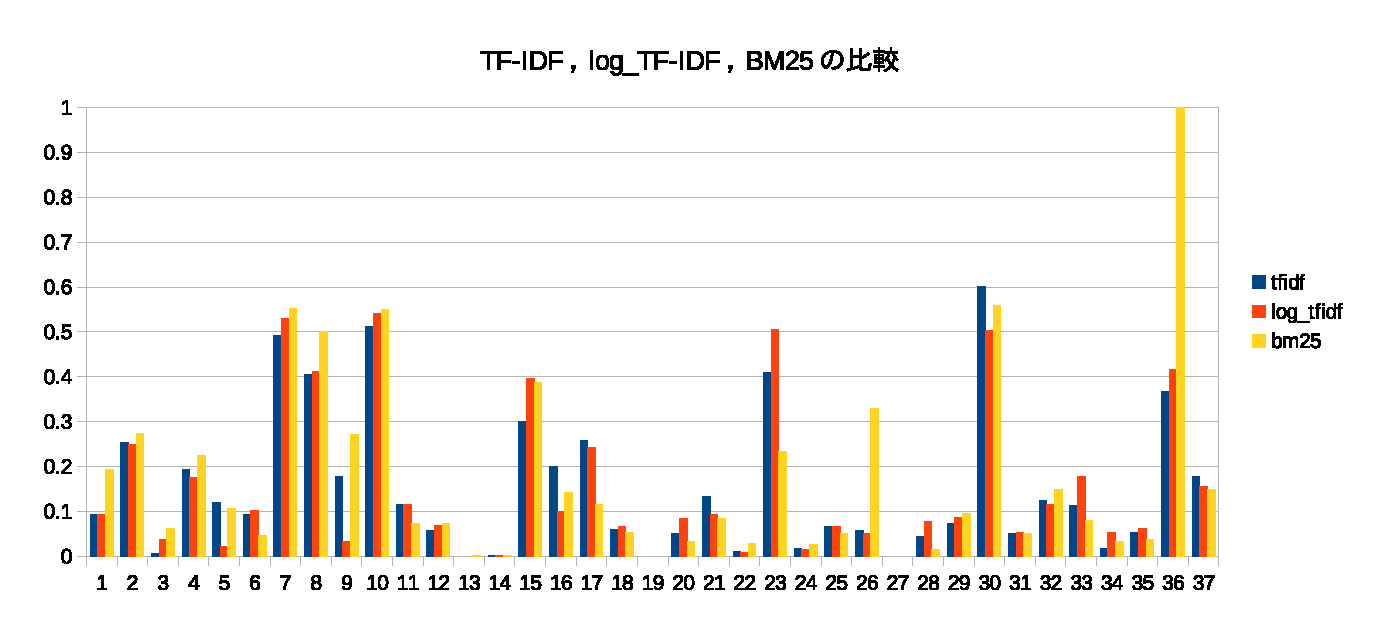
\includegraphics[width=7cm]{./graph/TFIDF_log_BM25.eps}
    \caption{TF-IDF, log\_TF-IDF, BM25のクエリ別検索精度}
    \label{fig_tf_log_BM25}
\end{figure}
表\ref{t_text}においてTF-IDFとlog\_TF-IDFのMAP値を比較すると,文書検索においてほぼ同等の性能があることがわかる.
ただし図\ref{fig_tf_log_BM25}から,log\_TF-IDFはTF-IDFより,正解文書が短いクエリに対して精度が良く,正解文書が長いクエリについてはTF-IDFより精度が下がる傾向があることがわかる.
一方でBM25はlog\_TF-IDFと同様の傾向があるが,一部のクエリにおいてTF-IDFの精度を大きく改善している.
これらのことから,TF-IDFにおいて文書長に応じてTFを正規化することにより,文書検索精度を向上させることができると考えられる.

\subsection{単語の意味的情報の加味}
\begin{figure}
    \centering
    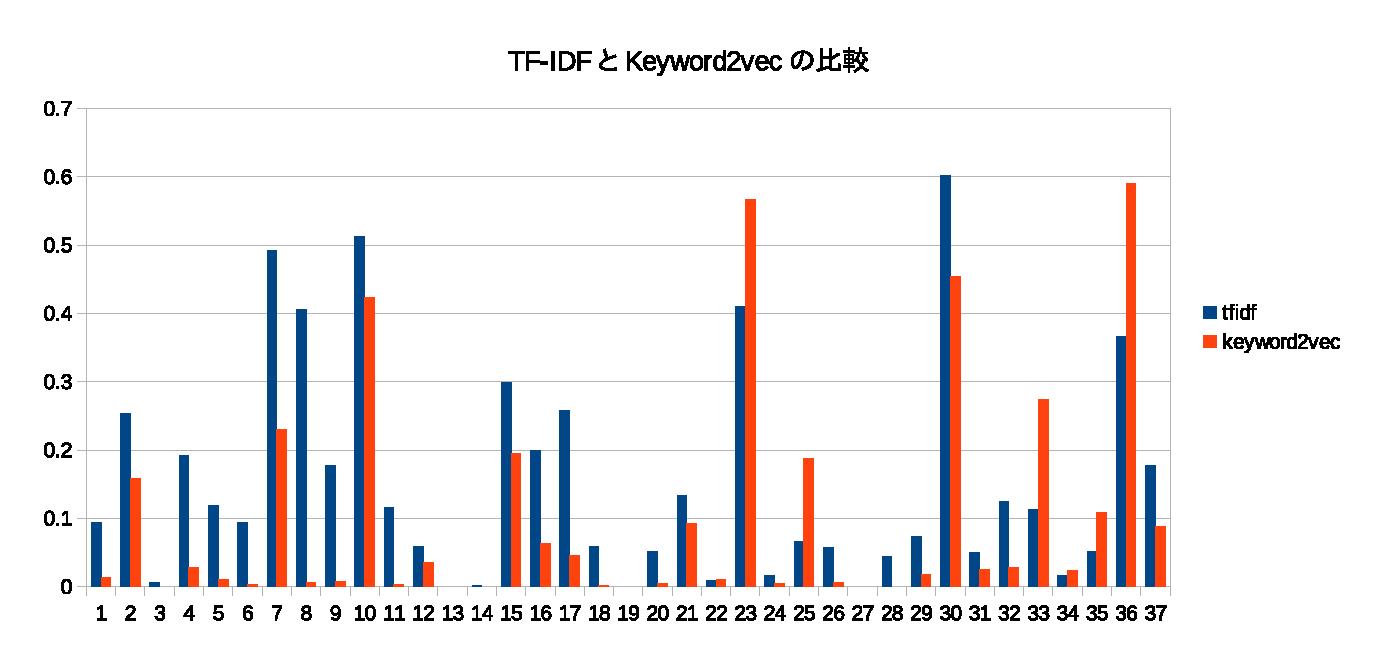
\includegraphics[width=7cm]{./graph/TFIDF_keyword2vec.eps}
    \caption{TF-IDF, log\_TF-IDF, BM25のクエリ別検索精度}
    \label{fig_tf_word2vec}
\end{figure}
表\ref{t_text}においてTF-IDFとword2vecのMAP値を比較すると,単語の意味的情報を考慮しないTF-IDFの方が優れた検索性能があることが分かる.
一方で図\ref{fig_tf_word2vec}から,word2vecは全体の精度では劣るが,一部のクエリにおいてTF-IDFを大きく上回る検索精度を示していることが分かる.
よって\ref{sec_word2vec}節に示した検索法は,従来法との組み合わせにより検索性能を大きく向上させることが
できると考えられる.

\subsection{部分文書検索における文書全体の情報の加味}
$\alpha = 0.9$のとき,表\ref{t_text}よりMAP値が最大値0.2745となった.
これは部分文書検索において,文書全体の情報を用いることが精度向上に大きく貢献することを意味する.

\subsection{音声認識誤りの棄却}
\begin{table}[htbp]
    \begin{center}
        \caption{音声認識結果を用いた文書検索精度}
        \begin{tabular}{|c|l|}
            \hline
                     &   MAP   \\ \hline
            棄却無し & 0.1067 \\ \hline
            棄却あり & 0.09406 \\ \hline
        \end{tabular}
        \label{t_spoken}
    \end{center}
\end{table}
音声認識結果のクエリ・文書を用いて文書検索を行った.
表\ref{t_spoken}に結果を示す.
表\ref{t_spoken}より,誤り棄却がある場合の方が逆に精度が劣化していることが分かる.
ここで誤り単語の棄却率は,FARが0.241,FRRが0.406であった.
このことから,認識誤り単語の棄却はできるが,その一方で検索に有用な語を棄却したため,精度が劣化したことが分かる.
しかし一方で,単語$w$を認識誤り単語とする$sumPMI(w)$の閾値を変化させることで,検索精度が向上する可能性があると言える.


%%%%%%%%%%%%%%%%%%%%%%%%%%%%%%%%%%%%%%%%%%%%%
% 第7章分割

\chapter{結論} 
\section{まとめ}
本研究では,文書検索において検索精度に影響を及ぼす要因を4つ取りあげ,それらについて分析を行った.

まず,音声認識精度と検索精度に関しては,従来から使用しているJuliusによる音声認識結果より,高性能な音声認識システムであるKaldiを用いた音声認識結果を用いたときの方が,検索精度が上昇する事が確認できた.

クエリの関連文書を用いたクエリ尤度モデルの拡張では,論文を用いたときに,MAP値の向上が見られた.しかし,Web文書を用いたときは,MAP値にあまり変化が見られなかった.これは,Web文書がNTCIR11のクエリに対して,スムージングを行なえなかったためであると推察できる.論文を用いると,専門単語も広く言語モデルとして含められるため,スムージングできる可能性が高くなり,MAP値が上昇したのだと考えられる.

次に,前後の部分文書の情報の加味では,精度を大幅に向上することを確認した.今回のSpokenQuery\&Docは,1つのクエリに対する正解文書が,1箇所に固まっていることが多かったため,特に効果が大きかったと考えられる.

最後に,これまでに説明してきた手法の中で,検索性能の向上に有効な結果を示したものを統合し,検索精度の更なる向上を図った.その結果から,前後の部分文書の情報を加味した場合,MAP値は大幅に改善した.しかし,キャッシュモデルに前後の部分文書の情報を加味した場合,特徴量が重複してしまい,良い結果が得られなかった.

\section{今後の課題}
今後の課題としてまず,ディリクレスムージング時のパラメータの設定があげられる.今回は人手で調整し,MAP値が高くなる値を設定したが,今後は尤度関数を設定し,最適化することによりパラメータを調節したい.

TODO: その他, RNNとかKNが上手く行ってないところ,論文の精度が向上しないところ、キャッシュモデルとスライド統合が競合してしまっているところ

% 単語の意味的情報を,検索精度が向上するように従来の検索法に組み合わせることが挙げられる. word2vecを用いた文書検索法は,TF-IDFの検索精度が高くないクエリにおいて大きく精度を向上させる傾向があったため,
% 互いの欠点を補い合うような組み合わせ方をすることで,精度向上に繋がるのではないかと考えられる.

% 音声認識誤りの棄却において,棄却の閾値を変化させた場合にどのように精度が変化するのかを確認しなくてはならない.
% 検索に有用な語を棄却してしまったため,閾値を負に設定することで,棄却の厳しさを緩和させることができる.
% また$sumPMI$が負になりやすい語に,何かしらの傾向が見られないか調査することで,検索に有用な語を棄却する問題を解決できると期待できる.

% 最後に,本研究で取り上げた手法を複数組み合わせることで,検索精度がどのように変化するか確認することが重要である.
% 本研究では要素を1つ1つ取り上げ,それぞれを独立に実験した.
% 一方でこれらの手法は組み合わせることができる.これらの手法を組み合わせることで,更なる精度の向上が期待できる.



%% 謝蟞
\onecolumn %1段組にする
% 第何章 といった見出しを出さない. #-> \chapter*
% 上記のことを満たしながら,目次は出す #-> \addcontentsline
\chapter*{謝辞}
\addcontentsline{toc}{chapter}{謝辞}
本稿をまとめるにあたり,多くの方々のお世話になりました.以下に感謝の意を表します.

% % 先生方
本研究のテーマを与えてくださり,温かいご指導を賜った,速水 悟教授,田村 哲嗣助教に深く感謝致します.
速水 悟教授には,研究の方針に関して普段から厳しく,かつ的確なご指導を頂きました.
田村 哲嗣助教には,研究の方針はもちろんのこと,研究の進捗に気を配って頂きました.
お二人のバックアップがなければ,本稿をまとめられることはありませんでした.

また,当研究にご協力いただいた速水・田村研究室のメンバーである竹原正矩氏,加島卓磨氏,川嶋大義氏,絹田卓也氏,臼田寛明氏,野尻弘也氏,鵜飼和渡氏,中嶋航大氏,朝日翔太氏,小川和晃氏,小島聖司氏,丹羽高大氏,藤原正希氏,松井智哉氏,宮崎晃一氏,村橋達明氏,山田詩織氏に感謝の意を捧げます.

% % 研究に深く関わってくれた人
% 次に研究の過程で,度々議論を交わし意見を頂きました竹原 正矩氏,川\UTF{7028} 徹也氏,田口 拓明氏,中嶋 航大氏に感謝の意を表します.
% 皆様には先生方とのミーティングの合間に,研究の結果について深く議論を交わし,多くのアドバイスを頂きました.
% 特にNTCIRプロジェクトのタスク参加者として実験プログラムの開発,及び修正を手伝い,実験の協力をして頂きました田口 拓明氏,
% 同じく実験の協力をして頂きました中嶋 航大氏には,より一層の感謝の意を表します.
% % 長谷川先輩
% また音声ドキュメント検索の研究の先駆者であるOBの長谷川 貴一氏には,多忙の中研究室にお越し頂き,
% 文書検索に関する多くのアドバイスを頂きました.ここに感謝の意を表します.\\

% % 研究室5階メンバー
% 速水・田村研究室E522のメンバーの
% 森長 夕貴氏,臼田 寛明氏,加島 卓磨氏,田口 拓明氏,絹田 卓也氏,井端 ひかり氏,葛谷 恵美氏,中嶋 航大氏には心より感謝致します.
% 出来のいい先輩ではありませんでしたが,本稿をまとめられるのは皆様の支えがあるからこそと認識しています.\\
% また同じ速水・田村研究室の現役の学生である,
% 竹原 正矩氏,
% 宇野 太久哉氏,河\UTF{FA11} 卓也氏,川\UTF{7028} 徹也氏,世古 拓海氏, 川嶋 大義氏,野尻 弘也氏,
% 鵜飼 和渡氏,廣瀬 彩恵氏,宮川 加奈子氏には,週二回のゼミで研究に対して意見を頂いたのみならず,
% 普段の研究活動においても多くのご支援を頂きました.
% ここに謝意を示します.\\

% % 秋葉先生,南條先生
% 豊橋技術科学大学の秋葉 友良先生には,NTCIR11 SpokenQuery\&Docのタスクにおいて貴重なテストコレクションを頂いたのみならず,
% NTCIR11 カンファレンスの場において貴重な意見を頂きました.
% また同様に龍谷大学の南條 浩輝先生とは,NTCIR11 カンファレンスの場において深い議論を交わし合いました.
% お二人に感謝致します.\\

% ソフトウェア開発
% 最後に,文書検索のシステム構築にあたり,形態素解析エンジンの部分には
% 京都大学情報学研究科−日本電信電話株式会社コミュニケーション科学基礎研究所 共同研究ユニットプロジェクトを通じて開発された
% MeCabを使用させて頂きました.
% また,3年間の研究活動の中でのプログラム開発において,Bram Moolenaar氏が開発されたエディタのVimを
% 使用させて頂きました.
% 本システムの構築にあたり,これらの優秀なオープンソースソフトウェアには大変お世話になりました.
% ご提供頂きました皆様に感謝致します.\\


% 速水 悟教授
% 田村 哲嗣助教
%
% 竹原 正矩氏
%
% 宇野 太久哉氏
% 川瀨 徹也氏
% 河崎 卓也氏
% 世古 拓海氏
% 原 謙介氏
% 森長 夕貴氏
%
% 臼田 寛明氏
% 加島 卓磨氏
% 川嶋 大義氏
% 田口 拓明氏
% 絹田 卓也氏
% 野尻 弘也氏
%
% 井端 ひかり氏
% 鵜飼 和渡氏
% 葛谷 恵美氏
% 中嶋 航大氏
% 廣瀬 彩恵氏
% 宮川 加奈子氏


%%%%%%%%%%%%%%%%%%%%%%%%%%%%%%%%%%%%%%%%%%
%%  参考文献

% \begin{thebibliography}{99} % 10件以䞊の堎合99を指定

% \renewcommand{\bibname}{参考文献}

% % NTCIR
% \bibitem{NTCIR}
% NTCIR \\
% \url{http://ntcir.nii.ac.jp/jp/about/}
% % MeCab
% \bibitem{MeCab}
% 圢態玠解析゚ンゞン MeCab \\
% \url{http://mecab.googlecode.com/svn/trunk/mecab/doc/index.html}

% \bibitem{ChaSen}
% 圢態玠解析゚ンゞン 茶筌
% \url{http://chasen-legacy.sourceforge.jp/}

% \bibitem{BM25}
% S. Robertson and H. Zaragoza, 
% The Probablistic Relevance Framework: BM25 and Beyond, 
% Foundations and Trends in Information Retrieval, Vol. 3, No. 4, pp.333-389, 2009.

% \bibitem{query_likelihood}
% J.M.Ponte, W.B.Croft, A language modeling approach to information retrieval, 
% Proc. 21st Annual International ACM SIGIR conference on Research and Development in Information Retrieval, pp.275-281, 1998.

% \bibitem{word2vec}
% T.Mikolov, K. Chen, G.Corrado, J.Dean, 
% Efficient Estimation of Word Representations in Vector Space, 
% arXiv:1301.3781, 2013

% \bibitem{convolutionalway}
% R.Collobert, J.Weston, A unified architecture for natural language processing: deep neural networks with multitask learning, 
% Proceedings of the 25th international conference on Machine Learning, pp.160-167, 2008

% \bibitem{turing}
% W.A. Gale
% Good-Turing smoothing without tears, Journal of Quantitative Linguistics Vol.2 pp217-237, 1995

% \bibitem{PMI}
% 浅芋倪䞀, 野本枈倮, 小橋川哲, 山口矩和, 政瀧浩和, 高橋敏
% 平滑化自己盞互情報量を甚いた音声ドキュメント認識信頌床の掚定, 日本音響孊䌚講挔論文集(秋) 2-10-3 pp.57-58, 2011

% \bibitem{IR_research}
% 江口 浩二, 情報怜玢のための確率的蚀語モデルに関する動向ず課題, 電子情報通信孊䌚誌, D Col.J93-D No. 3 pp.157-169, 2010

% itunes
% \bibitem{itunes}
% iTunes:
% \url{http://www.apple.com/jp/itunes/features/}

% \end{thebibliography}

% 付録
% \chapter*{発表文献}
% \addcontentsline{toc}{chapter}{発表文献}
%
\renewcommand{\bibname}{発表文献}
\begin{thebibliography}{99} % 10件以上の場合99を指定

\bibitem{asj2013}
原 謙介, 関谷 秀樹,  田村 哲嗣, 速水 悟, \\
Web情報に基づく認識信頼度の推定とキーワード抽出, \\
日本音響学会 春季研究発表会, 3-P-27c, pp.235-236, 2013 

\bibitem{apsipa}
K. Hara, H. Sekiya, T. Kawase. S. Tamura, S. Hayamizu, \\
Confidence estimation and keyword extraction from speech recognition result based on Web information, \\
In proceedings of APSIPA 2013

\bibitem{ntcir}
K. Hara, H. Taguchi, K. Nakajima, M.Takehara, S.Tamura, S.Hayamizu, \\
Segmented spoken document retrieval using word co-occurrence information, \\
In proceedings of NTCIR11, 2014

    
\end{thebibliography}


\end{document}
